\section{Experiments (OLD)}
\label{sec:experiments2}

We study the following questions. \\
\noindent
\textbf{1. Performance.} What is the approximation bound in practice, compared with the worst case guarantee given by Theorem \ref{theorem:algo}? How does the solution quality (in terms of the $\expinf{}$ objective) compare with other baselines, for the single stage version, i.e, $\mathcal{T}=\{0\}$?\\
\noindent
\textbf{2. Impact of time on the quality and structure of solution.} How does the objective value increase from a single stage to two stage? What kinds of nodes are picked in each stage?\\
\textbf{3. Interplay between information delay and intervention time.} Do we gain by waiting for information about the outbreak? By how much? At what point is it better not to wait?

% 1. What is the benefit of performing two stage non-adaptive interventions in comparison to the single stage strategies?

% 2. What is the impact of delay $\tau$ in the solutions to \probdelay for a fixed intervention time $T$ and budget $B$?

% 3. Given the delay in information $\tau$, how long can the policy makers wait for the information to perform the intervention? 

% 4. How does our algorithm perform on the montgomery network? What kind of people are picked for intervention for non-adaptive strategy with budget split? 

\subsection{Dataset and Methods}
We experiment with four very different kinds of networks, two random and two real, in order to fully explore the effect of network structure on the the results. We consider two random networks, namely the small world 
\cite{Kleinberg00thesmall-world}, and preferential attachment \cite{Barabasi509} models. We also study the results on the CA-GrQc collaboration network \cite{Leskovec:2007:GED:1217299.1217301}, since it is a type of social network. Finally, we consider a synthetic agent based population for Montgomery County, VA, constructed by a first principles approach by \cite{barrett:wsc09,eubank:nature04}. This has been used in several public health studies, e.g., \cite{singh:bmc19}. This network has a rich set of demographic attributes for each node, e.g., age, gender, and income.

\noindent
\textbf{Methods.}
We use \algo{} with one time step (i.e., $\mathcal{T}=\{0\}$, also referred to as single stage), or two time steps (i.e., $\mathcal{T}=\{0, T\}$, referred to as two stage, with $t=0$ being the first stage, and $t=T$ being the second stage). In the experiments involving delay, we use \algodelay{} with various $\tau$ and $T$ values. For the single stage problem, we use the strategy of picking nodes based on highest degree or eigenscore, which is the component in the first eigenvector of the graph's adjacency matrix \cite{tong:cikm12}.
There are no prior baselines for temporal vaccination. 



% The description  of datasets used in our experiments in presented in Table \ref{tab:datasets}. The Montgomery dataset is the social contact network of the population in the Montgomery County, VA. The nodes in this network corresponds to the people, while the edges correspond to the interaction of a pair of people that spans over 6 hours. CA-GrQc \cite{Leskovec:2007:GED:1217299.1217301} is a collaboration network, where the nodes correspond to the authors submitting papers to General Relativity and Quantum Cosmology category of Arxiv. An edge between two authors represents a collaboration between the authors. Both the Small World and the Preferential networks are random graphs generated using packages available in Networkx\cite{osti_960616}. The Small World is based on Kleinberg's small-world model \cite{Kleinberg00thesmall-world}, generated using ``navigable\_small\_world\_graph" function with the parameters $n = 50, p = 1, q = 5, r = 2, dim = 2$. Preferential is a random graph based on the preferential attachment model\cite{Barabasi509}, generated using ``barabasi\_albert\_graph'' function with the parameters $n=1000, m=2$.


\begin{table}[!h]
\centering
\begin{tabular}{llll}
\hline
 \textbf{Dataset} & \textbf{Nodes} & \textbf{Edges}   \\ \hline
 Montgomery & 70729 & 198138 \\
 CA-GrQc & 5242 & 14496\\
 Small World (SW) & 2500 & 14833 \\   
 Preferential (PA) & 1000 & 1996 \\ \hline
\end{tabular}
\caption{Description of datasets}
\label{tab:datasets}
\end{table}

\subsection{Performance}
We find that the approximation guarantee is a small constant in practice. This is shown in Figure \ref{fig:approx}, which compares the objective value of \algo{} with the fractional LP value, which is a lower bound on the optimum cost. In Figure \ref{fig:baseline}, we find that \algo{} gives a significant improvement over the baselines, in terms of the expected outbreak size.
\begin{figure}[!h]
    \centering
    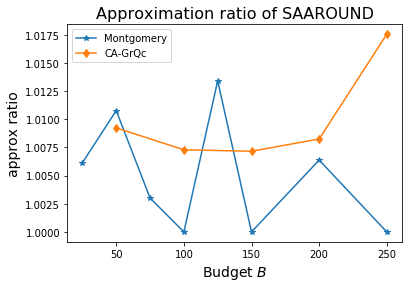
\includegraphics[scale = 0.35]{figures/approx.png}
    \caption{Approximation Ratio of \algo{} on real datasets.}
    \label{fig:approx}
\end{figure}
 

\begin{figure}[!h]
    \centering
    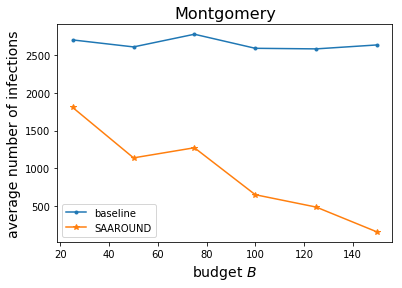
\includegraphics[scale = 0.5]{figures/baslinecomp.png}
    \caption{Montgomery. Comparison of \algo{} performance with degree based greedy algorithm as baseline. X-axis corresponds to the budget $B$ on the interventions, while the Y-axis corresponds to the average number of infections over all simulations. 
    }
    \label{fig:baseline}
\end{figure}
 
 
\subsection{Two stage interventions}
We study the two stage version of \prob{}. Here no information about the outbreak is available, and so, clearly, earlier is better, i.e., if the entire budget is available at time $0$, it is better to use it right away. In Figure \ref{fig:temporal}, we examine how the objective value $\expinf{}$ increases with $T$ in a two stage intervention, where $T$ is the time of the second stage. We observe that $\expinf{}$ increases very rapidly with $T$.

Next, we examine the structure of the sets picked in each stage. Figure \ref{fig:montagedeg} shows a scatter plot of the node degree and age of the solution to a two stage version with $T=4$. We observe that there are slight differences between the sets $X_0$ and $X_4$: $X_0$ has slightly higher degree nodes, whereas $X_4$ has slightly lower age nodes. But more importantly, \emph{it is not the case that all high degree nodes are used in $X_0$}.

% We call the intervention strategy without any information on the epidemic state as non-adaptive interventions. In such strategies, we can do at all interventions at a particular time step $T$ or do it at multiple time steps with the budget split over these times. In our experiments, we present the latter case for performing interventions at two time steps: (i) one set of interventions at $T = 0$ with $B/2$ budget and (ii) another set of interventions at $T = t$ with the remaining budget.
\begin{figure}[!h]
    \centering
    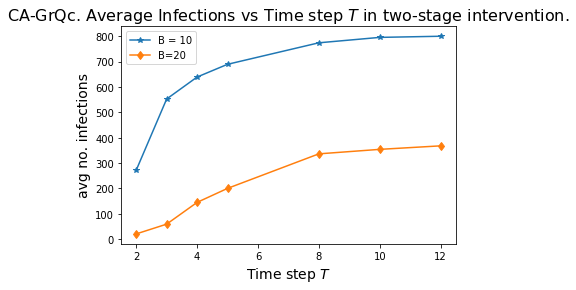
\includegraphics[scale = 0.4]{figures/twostage.png}
    \caption{CA-GrQc. Impact of varying $T$ in Two-stage Intervention. The X-axis corresponds to time step $T$ at which 2nd intervention is performed (1st intervention is at T =0). The Y-axis corresponds to the average number of infections over the simulations.}
    \label{fig:temporal}
\end{figure}

\begin{figure}[!h]
    \centering
    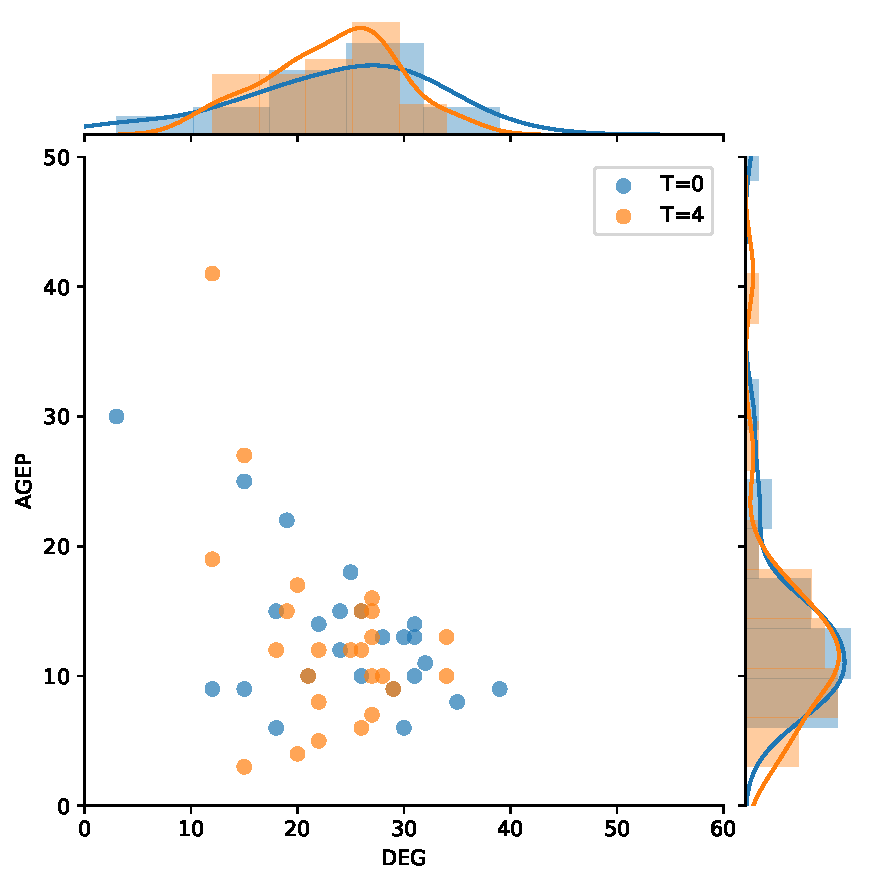
\includegraphics[scale = 0.45]{figures/t0_t4_compare_age_deg.pdf}
    \caption{Montgomery Graph: scatter plot of age and degree of nodes of the sets $X_0$ and $X_4$ in a solution to the 2-stage \prob{} with budgets $B_1 = B_4 = 25$.}
    \label{fig:montagedeg}
\end{figure}

\subsection{Interplay between information delay and intervention time}

Here, we consider the \probdelay{} problem, and study the interplay between the information delay $\tau$ and the time $T$ at which the intervention is done. 

\begin{figure}[!h]
    \centering
    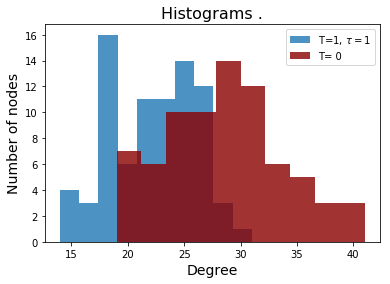
\includegraphics[scale = 0.6]{figures/histogram.png}
    \caption{X-axis corresponds to degree of nodes picked for intervention at $T=0$. Y-axis corresponds to number of nodes. The histogram in blue corresponds to node picked for intervention at $T = 1$ with $\tau = 1$. The histogram in dark red corresponds to the picked for intervention at $T = 0$.}
    \label{fig:hist}
\end{figure}


\subsubsection{Impact of delay in information}
\begin{figure}[!h]
    \centering
    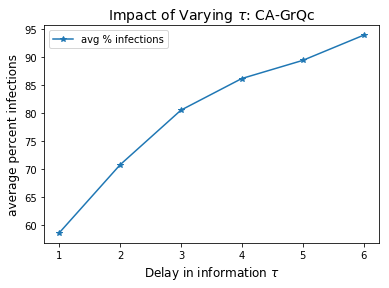
\includegraphics[scale = 0.5]{figures/varytauGrQc.png}
    \caption{Impact of varying $\tau$ for fixed T = 7 and B = 50: CA-GrQc}
    \label{fig:T7tau}
\end{figure}

We study the impact of delay of information $\tau$ for a fixed budget $B$ and time of intervention $T$. Figure \ref{fig:T7tau} shows that the average \% infected increases with the increase in $\tau$ value, for a fixed $T = 7$ and budget $B=50$. The average percentage infections is the average of the percentage of infections over the simulations.


%We observe that as the delay $\tau$ increases, the number of infections increases rapidly. Figure \ref{fig:T7tau} shows this phenomenon on CA-GrQC network for a fixed time of intervention $T = 7$ and budge $B = 50$. The average percentage infections is the average of the percentage of infections over all the epidemic simulations. 


\subsubsection{How long to wait for information}
We use \algodelay{} to examine when it is beneficial to wait for information before intervention, when is it not, by varying $\tau, T, B$ in Figure \ref{fig:howlong} for the Montgomery county, PA and SW networks, respectively. In each figure,
the red dashed line corresponds to the expected number of infections, i.e., the $\expinf(\cdot)$ objective, if the intervention is performed at time $0$. Each curve corresponds to a different $\tau$ value, and shows the $\expinf(X_T)$ objective on the $y$-axis, and the time $T$ on the $x$-axis. As long as the curves are below the red dashed line, an intervention at that time, taking the delayed information into account, is better than doing it at time $0$.

The time at which the curves intersect the red dashed line varies by network. For the Montgomery county network, $T$ is close to 14. But it is much smaller for both the PA and SW networks, and for them it does not help to delay the intervention much. Interestingly, for the Montgomery county network, we find the time at which the intersection happens is actually past the peak, shown in Figure \ref{fig:howlong}. We present the average epicurve of Montgomery dataset in Figure \ref{fig:epicurve}.


% In this section, we discuss when is it beneficial to wait for information before intervention, when is it not. We present results on the Small World, Preferential, and the Montgomery datasets. We fix the budget to $B$ and run our algorithm for various choices of intervention time $T$ and $\tau$. In case of the Small World dataset, we observe that waiting for information beyond $T= 2$ when $\tau = 1$ is worse than performing interventions at the beginning. When $\tau = 3$, it is always better to perform interventions at the beginning. This can be seen in Figure \ref{fig:swdelay}, where the red dashed line, corresponding to the number of infections after performing intervention at $T = 0$ cuts the curve corresponding to $\tau = 1$ before $T = 3$.

% The average epicurve corresponding to the average number of infections at each time step over all simulations is presented in Figure \ref{fig:epicurve}. The peak is around time step $T = 4$. As shown in Figure \ref{fig:montgodelay}, it is beneficial to wait for information when the delay is small (i.e. $\tau \in \{2, 4\}$). Our experiments suggest that, in such population, it is beneficial to wait for information at least till before peak.

\begin{figure}[!h]
    \centering
    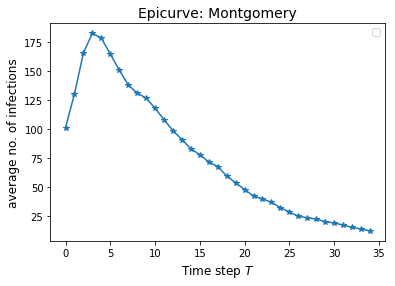
\includegraphics[scale = 0.5]{figures/epicurve.png}
    \caption{Epicurve for Montgomery: average number of infections at each time step $T$.}
    \label{fig:epicurve}
\end{figure}

\begin{figure*}[!h]

\centering
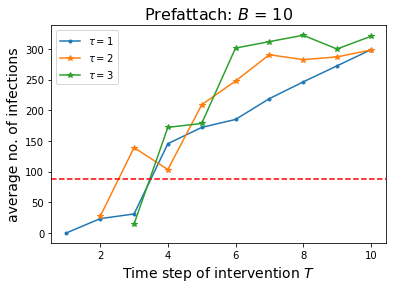
\includegraphics[width=.37\textwidth]{figures/prefattach_howlong.png}\hfill
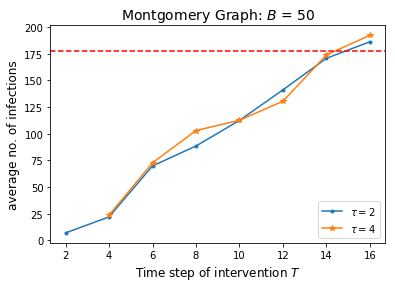
\includegraphics[width=.37\textwidth]{figures/montgo_howlong.png}\hfill
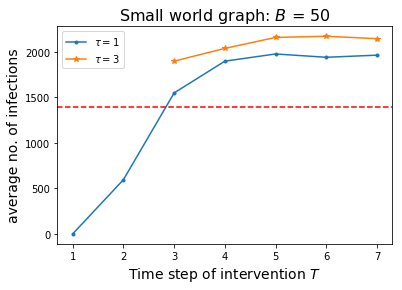
\includegraphics[width=.37\textwidth]{figures/sw_howlong.png}

\caption{How long to wait for information? In each plot, X-axis corresponds to the time of intervention. Budget $B = 10$. Y-axis corresponds to the average number of infections. The dashed horizontal red line corresponds to the number of infections if the intervention is performed at the beginning of the epidemic.}
\label{fig:howlong}

\end{figure*}



